\Introduction
В 2019 году произошел запуск космической обсерватории СРГ (Спектр-Рентген-Гамма) с телескопами 
eROSITA и ART-XC на борту. Основной задачей этих телескопов является создание обзора всего неба в 
рентгеновском диапазоне. Данные, полученные от этих телескопов будут использоваться для обнаружения 
астрономических объектов трёх категорий:

\begin{enumerate}
    \item Скопления галактик.
    \item Сверхмассивные чёрные дыры.
    \item Рентгеновские звёзды в галактике Млечный путь. 
\end{enumerate}

Полные обзоры неба, полученные телескопом eROSITA, появятся к июню 2020 года, поэтому на данный 
момент есть возможность подготовить модели для сегментации данных на примере других диапазонов.\\

В первую очередь будут использоваться данные оптического диапазона. Видимое излучение --- тот 
диапазон частот, что доступен глазу человека. На текущий момент существует большое количество 
оптических телескопов, и, как следствие, большое количество данных, извлеченных с их помощью. В 
данной работе будут использоваться данные телескопа Pan-STARRS1, который является частью системы 
телескопов Pan-STARRS (Panoramic Survey Telescope and Rapid Response System). Этот телескоп 
построен на вершине гавайского вулкана Халеакала. На 2007 год он обладал самой большой 
светочувствительной матрицей в мире. Кроме того, его данные находятся в общем доступе \cite{Panstarrs}.\\

В последние годы методы глубокого обучения стали играть важную роль в анализе данных. Нейросетевые 
модели показывают высокие результаты в области компьютерного зрения и в частности в задачах 
сегментации и детекции. Всё более часто они применяются и для решения задач астрофизики. 
Характеристики телескопа eROSITA позволят получить рентгеновские данные очень высокого качества (то 
есть с низким количеством шума), и методы глубокого обучения дают много преимуществ при анализе 
данных: 

\begin{enumerate}
    \item Алгоритмы, не использующие нейросетевые методы, обычно требуют тонкой настройки и подбора 
        параметров, подходящих под характеристики данного телескопа и данной области неба. Нейросеть 
        же не требует предварительной настройки, и при достаточном количестве тренировочных данных 
        сможет одинаково хорошо сегментировать данные, для которых другим алгоритмам потребовались
        разные параметры.
    \item Аналогичнные методы можно использовать для сегментации одновременно разнородных данных. 
        То есть для улучшения качества сегментации можно исследовать параллельно разные диапазоны 
        частот и находить взаимосвязь между разными спектрами.
\end{enumerate}

На данный момент архитектура U-net \cite{Unet} является одной из лучших нейросетевых моделей для сегментации. 
Её симметричная структура позволяет абстрагировать данные изображения, подаваемого на 
вход, в то время как skip-connection слои помогают увеличивать точность сегментации.

\begin{figure}[h]
    \center{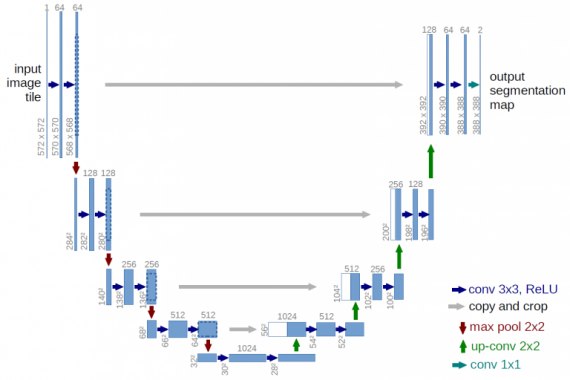
\includegraphics[width=0.7\linewidth]{unet0}}
    \caption{Структура модели U-net \cite{Unet}}
\end{figure}


